\documentclass[11pt, oneside]{article}
\usepackage{geometry}
\geometry{letterpaper}
\usepackage{graphicx}
\usepackage{amssymb}
\usepackage{algorithm}
\usepackage{algorithmic}
\usepackage{mathtools}
\DeclarePairedDelimiter\ceil{\lceil}{\rceil}
\DeclarePairedDelimiter\floor{\lfloor}{\rfloor}
\usepackage{pgfplots}
\pgfplotsset{width=10cm,compat=1.9}

\def\BibTeX{{\rm B\kern-.05em{\sc i\kern-.025em b}\kern-.08em
    T\kern-.1667em\lower.7ex\hbox{E}\kern-.125emX}}


\begin{document}
\title{Smart Prompt}
\author{Blake Patterson}
\date{August 1, 2022}
\maketitle

\begin{abstract}
Smart Prompt is an Alexa Skill aimed at helping those with memory issues keep better track of their daily/weekly tasks that they may otherwise forget to complete. 
It also keeps a record of those tasks and their completion times to better inform the individual and/or caregivers of how often the individual completes their tasks as well as how long it takes them. 
\end{abstract}

\pagenumbering{roman}
\newpage
\tableofcontents
\newpage
\pagenumbering{arabic}


\section{Introduction}

In 2002 in the US, as many as 3.4 million people above the age of 71 had dementia \cite{b4}. 
Not only are there no effective treatments for these impairments, but the number is not going down either. 
Due to this, many older adults are finding themselves unable to complete their basic tasks such as exercising, taking medicine, walking the dog, etc.
However, it is often not the case that they are physically and/or mentally unable to complete these tasks, it is simply a matter of forgetting about them. 
Thus, all these individuals need is someone or something to remind them to complete these tasks, and having someone there to remind them all day long is often not realistic, so it is only natural to look towards technology as a solution. 

One major problem with this, however, is that the vast majority of the people with memory impairments are not tech savvy. 
Thus, making some fancy mobile app with a bunch of bells \& whistles is more of a hinderance for them than a solution due to the learning curve. 
There is, however, one piece of technology that does not require a learning curve while still providing the functionality we need, and that would be Amazon Alexa. 
Alexa not only has a reminder framework that would allow us to build a solution to this problem, but can be interacted with solely through voice commands allowing for a non-tech savvy person to have a completely natural conversation with it. 
Not only that, but it is fairly common for any given household in America to have an Alexa enabled device of some sort in their home, allowing for easier adoption. 

With this in mind, we build an Amazon Alexa Skill called Smart Prompt to solve the problem many older Americans are facing by reminding users to complete their daily tasks. 
In addition, it has two unique functionalities to set it apart from standard reminders: personalization and the recording of tasks. 
Personalization (i.e., referring to the user by name \& playing custom audio upon completing a task) makes Smart Prompt more enticing to use as well as encourages the user to complete their tasks. 
Recording of tasks allows users \& caregivers of users to be fully aware of whether or not the user completed their important tasks (i.e., whether or not the user took their morning medicine). 

For the remainder of this paper we will examine existing solutions to this problem, examine our solution \& how it works, and finally compare our solution to what already exists. 


\section{Related Work}

\subsection{Feasibility Studies}

Let us start by examining some studies \& reports on the feasibility of using Alexa, other voice command interfaces, and other related technologies as a solution for reminding elderly patients (with \& without dementia) about their daily tasks as well as just helping them get about their daily lives. 

The first study is focused on examining how older adults who are not technologically proficient use voice assistants like Alexa \cite{b1}. 
There were no special Alexa Skills, mobile apps, or anything else developed for this study. 
There was also no targeted functionality of voice assistants that this study focused on, i.e., they were examining voice assistants as a whole and not just the reminder aspect of them. 
Additionally, they did not focus in on a specific user group aside from elderly individuals. 
In terms of their study, they deployed an Amazon Echo Dot \& Fire tablet into the homes of seven individuals above the age of 65 for three weeks. 
None of the participants had prior experience with voice assistants, none were proficient with computers in general, and many lived on their own. 
The researchers conducted a setup procedure with each participant, regular interim interviews, an exit interview, and also had the participants keep diaries of their experiences. 
In terms of results, all of the participants ended up growing comfortable using the Alexa device and were willing to keep using it after the study. 
Many of them had concerns at the beginning, but it was reported that these concerns had vanished by the end. 
Some participants even reported that, on occasion, it was easier to talk to Alexa as it would not get tired of repeating things and answering simple questions. 
In the end, however, there were two things to make note of, using a set launch command was not easy for many of the participants and they did not end up using reminders all that much. 
Having to say Alexa prior to everything ended up being very difficult for the users. 
Many of them used the wrong launch phrase during the first week, and at least one even continued to switch up the launch phrase with other words for the entire study. 
This could be a major issue for Smart Prompt as a custom Alexa Skill requires the user to not only say Alexa, but also say the skill name before everything they do. 
The other issue is that the participants simply did not really use Alexa for setting reminders. 
This could be for many different reasons, but considering the target user base for our problem is looking specifically for a reminder focused solution, it should not be a major issue. 

The next study again focuses on adding Alexa devices into the households of elderly individuals, but this time focuses on the actual impact it could make on their lives rather than just, "will \& can they use it" \cite{b2}. 
This study focuses on using Alexa to increase the amount at which patients adhere to their medicine, something much closer to what we are looking for in our solution. 
However, it is worth noting that they are less focused on reminding users with memory ailments to take their medication and more focused on making users more informed about their health and helping them know what medication to take and when. 
In short, they are looking to streamline and improve the way medication instructions are given. 
That is not to say they are ignoring the aspect of using Alexa to set reminders, as they are, it is just not their main focus. 
Similar to the first study, they gave the devices to 58 older individuals, the vast majority having long-term health issues. 
They conducted interviews at setup time, during the study, and two to three months afterwards. 
The results \& feedback was generally positive, and participants specifically liked the Alexa reminder \& list functionalities. 
In the end, this further reassures us that older individuals are willing \& able to use Alexa, and even proves to us that, at least when it comes to certain user bases, the reminder functionality of Alexa is a big hit. 

The final feasibility study explores a much broader topic, that being technology for elderly dementia patients in general, however it does touch upon Amazon Alexa and its applications to said patients a fair bit \cite{b6}. 
More specifically, it groups Alexa into the category of Smart Home devices, alongside other devices that connect to Alexa, safety sensors/devices for various household objects, automatic pill dispensers, and more. 
Although not so prevalent to our topic, it does bring up many benefits Alexa provides to these patients such as reminding them to turn off lights that they may have accidentally left on and allowing relatives \& caregivers who live elsewhere to connect their Amazon accounts, enabling them to be more connected \& helpful to the patient in question, even from a distance. 
While much of this does not directly related to the topic of reminding patients of their daily tasks, it proves there are countless other reasons for the patients to use an Alexa, and speculates on how it can tailor to each individuals needs rather than be something only useful to some patients. 

Overall, studies have shown that Alexa is surprisingly easy to pick up for elderly dementia patients, ends up being more helpful than they expect (even if it is in ways they did not intend), and can truly increase their quality of life by reminded them of things such as taking medicine. 
While there are definite cases of patients not getting used to Alexa, not finding it helpful, or just outright being against it, these results show that something like Smart Prompt is not only feasible, but likely to help many patients. 

\subsection{Design \& Discussion Studies}

Next let us examine two studies that discuss different aspects of using Alexa for dementia patients and focus more on the conclusions they draw that can help us design Smart Prompt. 

The first study here focuses on the broad category of intelligent cognitive assistants rather than Alexa specifically, and discusses the results of their focus groups to conclude on how to design a better intelligent cognitive assistant \cite{b7}.
Much like the other studies, they conducted three focus groups that simply consisted of dementia patients as well as their family members interacting with and using an intelligent cognitive assistant. 
Much of the details about the study and many of the findings remain similar to the other studies so it is not worth repeating, although there is one major conclusion worth bringing up. 
Seemingly one of the most important aspects of an intelligent cognitive assistant is personalization, just as we intend to implement with Smart Prompt. 
Essentially, they came to the conclusion that every patient was unique \& had different needs and wants (as any person does), and so to design a good assistant, it would need to be able to adapt to those different needs and wants. 
They go into some detail about how to personalize the assistant that goes beyond what is planned for Smart Prompt, although this further validates that personalization is an important feature for our solution. 

The other study is focused more on evaluating existing chat bots, as they call them, for dementia care \cite{b5}. 
Although chat bot is often not a term used to refer to an Alexa Skill, five of the six that they examined were Alexa Skills. 
Many of these skills were focused more on providing information about dementia rather than providing aid to a dementia patient, although there are still some useful findings here. 
Again, one of their biggest conclusions validates our need for personalization, the need for a human feel. 
They even go as far as to say that one of the skills passed the Turing test, and although that is a bit of a stretch, it is important to acknowledge that the more the user feels they are talking to a human, the more comfortable they will be. 
They also acknowledge that a human feeling chat bot that cannot do its job does not provide much benefit, so it still needs to serve some purpose and do it well, but they further stressed the importance of the human feel. 
The other main thing they stressed was the backing of a skill with evidence. 
This makes more sense for the information providing skills they were examining, although it is worth taking into account for Smart Prompt. 
The more evidence and concrete data we take into account when building Smart Prompt, the more useful it will be to patients. 

Overall, these studies further show that personalization is a must have for Smart Prompt, and we should continue to further humanize the skill as much as possible. 

\subsection{Remembranza Pills}

Finally, let us examine a real project. 
Remembranza Pills \cite{b3} is very similar to Smart Prompt in that it is an Alexa Skill built to help elderly patients remember to take their medicine. 
It works in three main stages: 
\begin{enumerate}
  \item A Doctor or caregiver adds all the necessary details of a patient's medication(s) via the connected web app, storing all of the information on the internet.
  \item The patient communicates with the Alexa Skill throughout the day in order to determine what medications to take at which times. This happens via the patient directly asking Alexa what medication to take, the skill does not remind the user automatically. The Alexa Skill also asks the patient whether or not they took the medication every time it tells them they should and records their answer.
  \item Finally, relatives, caregivers, or other relevant parties can use the Android app to monitor whether or not the patient has been taking the required medications. 
\end{enumerate}

This structure \& flow is very similar to the desired structure of Smart Prompt. 
It contains one of the two main points that are a must have for our solution, task completion recording. 
It also consists of supplementary apps, web \& mobile, for creating, updating, deleting, and monitoring reminders/tasks, which are components that have been planned to be added to Smart Prompt in the future. 

On the other hand, Remembranza is missing two big things that are requirements for Smart Prompt, personalization \& automatic reminders. 
The personalization is straight-forward, our solution should have some sort of incentive and personalized feel to make the patient more comfortable using it. 
Automatic reminders are somewhat less straight-forward, but an absolute necessity. 
The only way a patient can be reminded of what medicine to take with Remembranza is if they remember to ask Alexa what medicine they have to take. 
So, they are being relieved of having to remember exactly what medicine they need to take, but they are still expected to remember the fact that they have to take something. 
This is no good, as if they forget they have to take medicine in the first place (a highly likely situation for our user base), Remembranza will never remind them and they will most likely not take their medicine. 

Remembranza was implemented and successfully tested in a laboratory setting, however it was not directly tested by our target user base. 
As such, there are not many useful takeaways aside from what they set out to do is possible. 
Overall, Remembranza is a great start towards the solution we are looking for, it just does not quite meet all of our requirements. 


\section{Design}

Smart Prompt, at its core, serves a fairly straightforward purpose: it allows users to create and manage weekly reminders. 
To give more detail, a user is able to create a reminder to go off on a certain day of the week at a certain time, and that reminder will go off at that day \& time each week (until the user removes that reminder). 
Then, when a reminder goes off, the user is notified of the message that they asked the reminder to give, and they can then tell Smart Prompt once they have completed their task in order to mark it as complete. 
Finally Smart Prompt will send the user's smart phone a push notification alongside each reminder, so that they can see their reminders even if they are not at home. 

At a technical level, Smart Prompt consists of two parts: Amazon Alexa as a front end \& Google Firebase Realtime Database as a backend. 
Let us examine those two parts and how they contribute to this purpose. 

\subsection{Features}

Here is a complete list of features in Smart Prompt (More details about the features not yet implemented will be provided in the Discussion section).
\begin{center}
\begin{tabular}{| c | c |}
 \hline
 Feature & Status \\ [0.5ex] 
 \hline\hline
 Grant Permissions via Verbal Approval & Complete \\
 \hline
 Create Reminder & Complete \\
 \hline
 Refer to User by Name & Complete \\
 \hline
 Store User Data in Database & Complete \\
 \hline
 Store Reminder Data in Database & Complete \\
 \hline
 Recording a Reminder as Complete & Complete \\
 \hline
 Playing an Audio File Upon Task Completion & Complete \\
 \hline
 Managing Reminders (i.e., CRUD) & Complete \\
 \hline
 Manually Snooze Reminders & Complete \\
 \hline
 Auto Snooze Reminders & In-Progress \\
 \hline
 Web App for Managing Reminders \& Viewing Completion & TBD \\
 \hline
\end{tabular}
\end{center}

\subsection{Frontend}

The frontend, as explained before, is built using Amazon Alexa. 
In its simplest form an Alexa can be explained as a set of intents, i.e., actions for the users to perform with the skill, and the skill can do any number of things when an intent fires. 
There are also some outliers such as event \& request handlers, which can be viewed in a very similar light, with the major difference being that they are not usually fired from the user saying something. 
There are many more details than that, but let us go through the main intents (as well as some request \& event handlers) of Smart Prompt and what they do. 

\subsubsection{Launch Request}

This is simply what occurs when the skill launches, i.e., immediately after the user says, "Alexa, open Smart prompt". 
There is not much to speak of here, although this is where the necessary permissions are requested and granted the first time a user uses Smart Prompt. 
More specifically, Smart Prompt requires explicit permission from the user in order to create reminders for them as well as use their first name. 
Once the user has granted these permissions, the skill will simply ask them what they would like to do. 
Once the permissions are granted, every proceeding launch request will skip straight to asking the user what they would like to do. 

Here is what the launch request looks like:
\begin{center}
  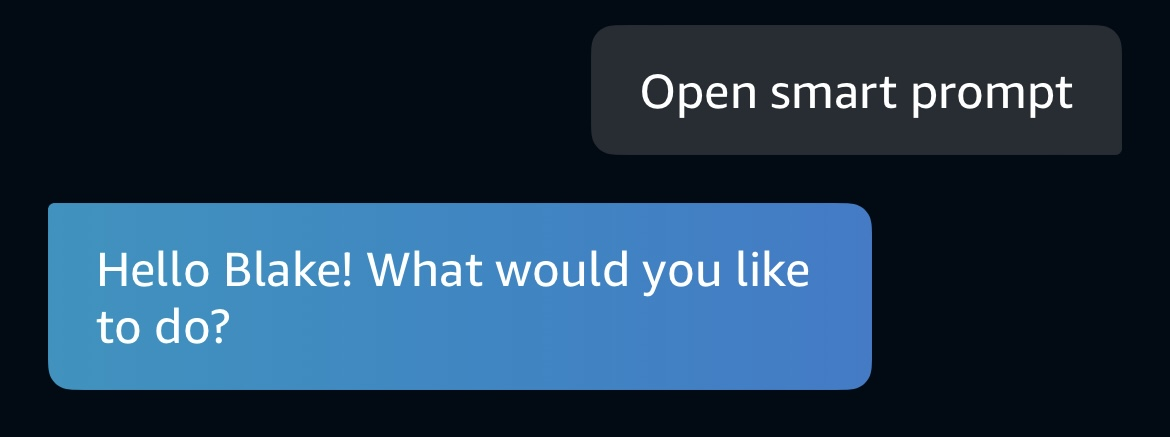
\includegraphics[width=\linewidth * 3/4]{images/launchRequest.jpg}
\end{center}

\subsubsection{Create Reminder Intent}

The Create Reminder Intent, as one would assume, allows the user to create a reminder. 
Ideally reminders would be set up early on (possibly even by a caregiver or an expert prior to the user ever interacting with the skill), so a user should not have to use this intent often, although it is there for whenever they need to quickly set up a new reminder. 

The Create Reminder Intent takes in three required slots, i.e., small bits of information provided by the user for processing. 
The three slots are the day of the week the reminder should take place on (i.e., Sunday, Monday), the time of day the reminder should go off (i.e., 9am, noon, 3pm), and finally the message the reminder should give (i.e., "walk the dog", "take medicine").
The intent can collect these three pieces of information in multiple different ways. 
The user could start by providing no information other than that they want to create a reminder, and the skill will prompt them for each slot individually. 
They can also provide the day, the time, or the day and time up front, in order to skip the tedious process of Alexa asking them for that. 
Finally, they can also just provide the reminder message. 
Whatever slots they do not provide up front will simply be collected via additional prompts given by the skill. 
As one final check once the slots are gathered, the skill will read them back to the user and ask if they are correct, giving the user one final chance to cancel in case Alexa interpreted something incorrectly. 
This varied way of creating a reminder allows for a much more natural feeling interaction with the skill. 

After collecting all of the slots and confirming they are correct with the user, the skill will go ahead and do two main things: create the reminder using the Alexa Reminders API \& register the skill in the database. 
The database will be discussed further in the backend portion of this section, but there is one important thing to note about how the reminders are created with the API. 
When the reminder is created, it is actually creating multiple reminders at once, one for the initial reminder and one for each snooze that should take place if the user does not record it as complete. 
This is done due to technical limitations of not being able to update the one reminder's time automatically at certain points of the project's execution cycle. 
Everything else about the creation of the reminder(s) is fairly straight forward, all of the information collected along with some other boiler plate information is send through an API request to Alexa's system and the reminder is created.
If for whatever reason this fails at any point (considering it is an API request as well as a database operation), the user is notified of the failed creation and asked to try again. 

Here is one example of how to create a reminder:
\begin{center}
  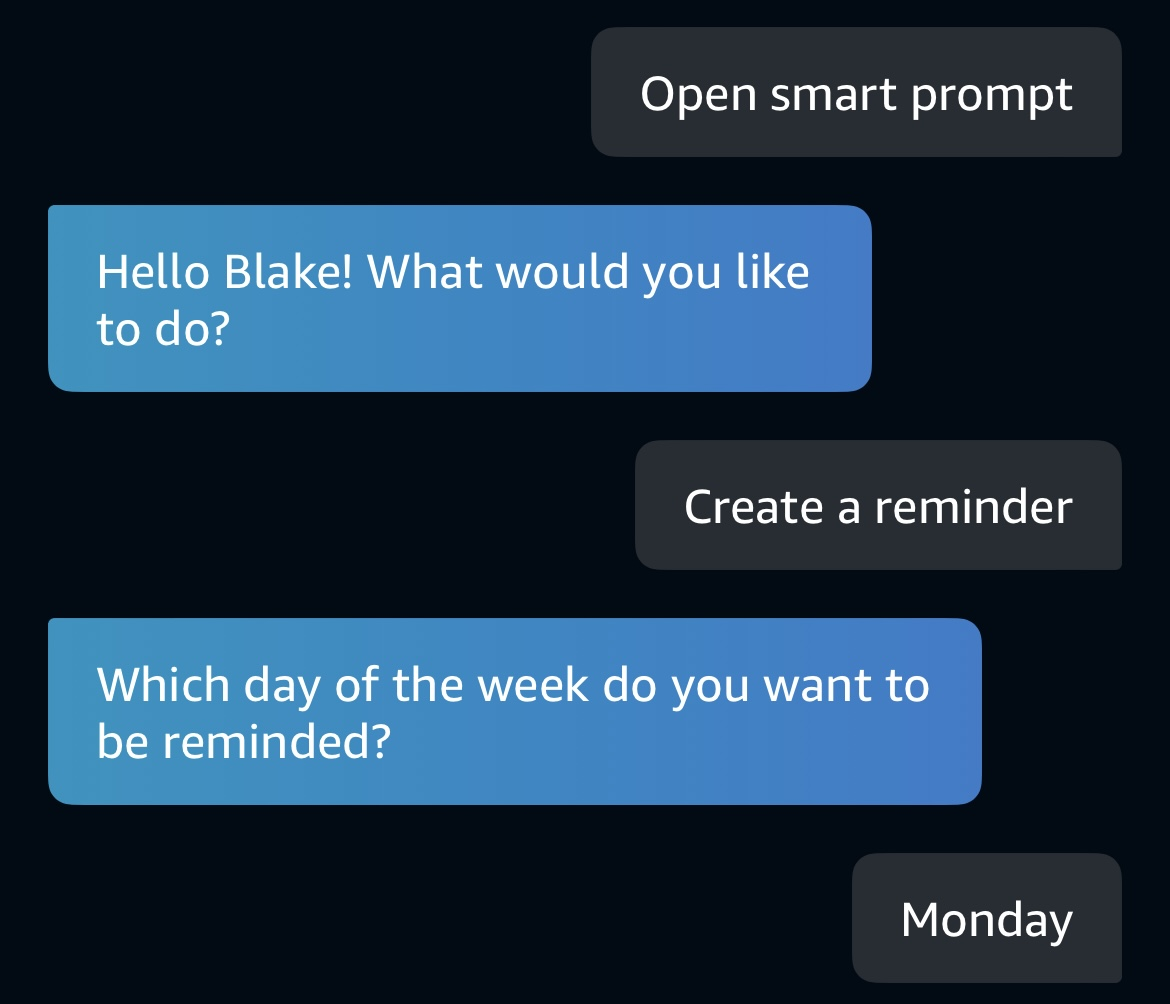
\includegraphics[width=\linewidth * 3/4]{images/createReminder1a.jpg}
\end{center}
\begin{center}
  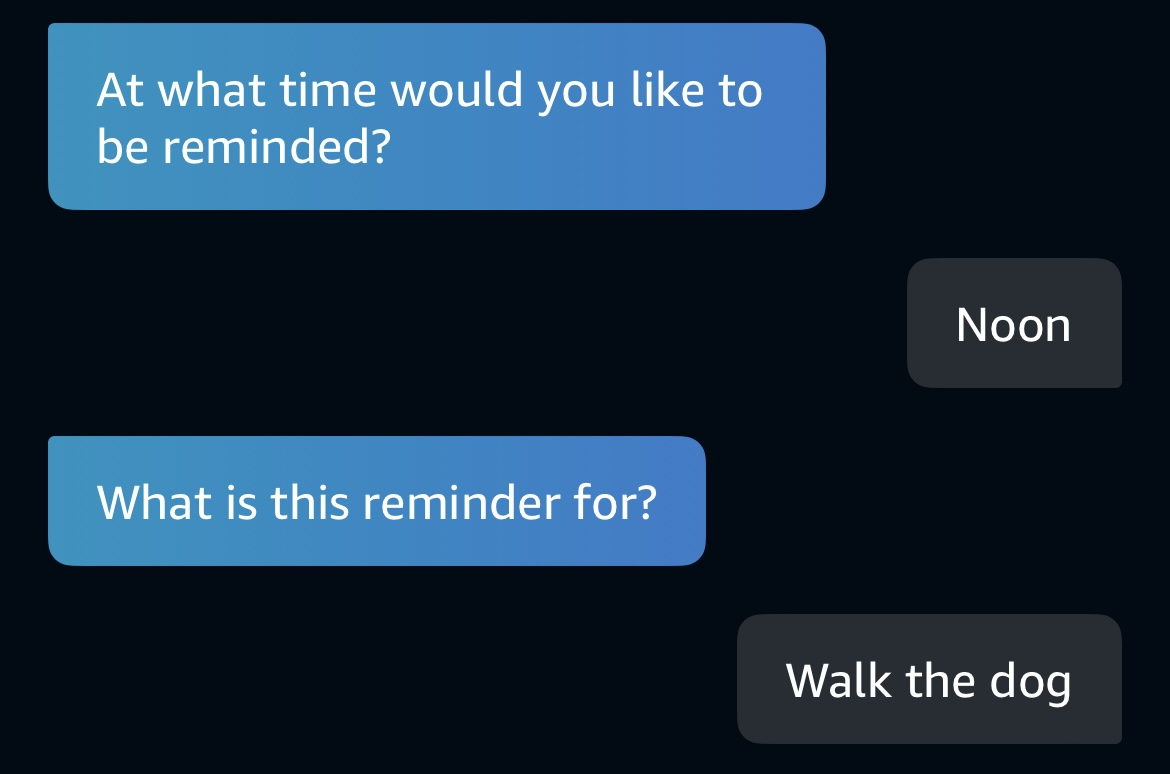
\includegraphics[width=\linewidth * 3/4]{images/createReminder1b.jpg}
\end{center}
\begin{center}
  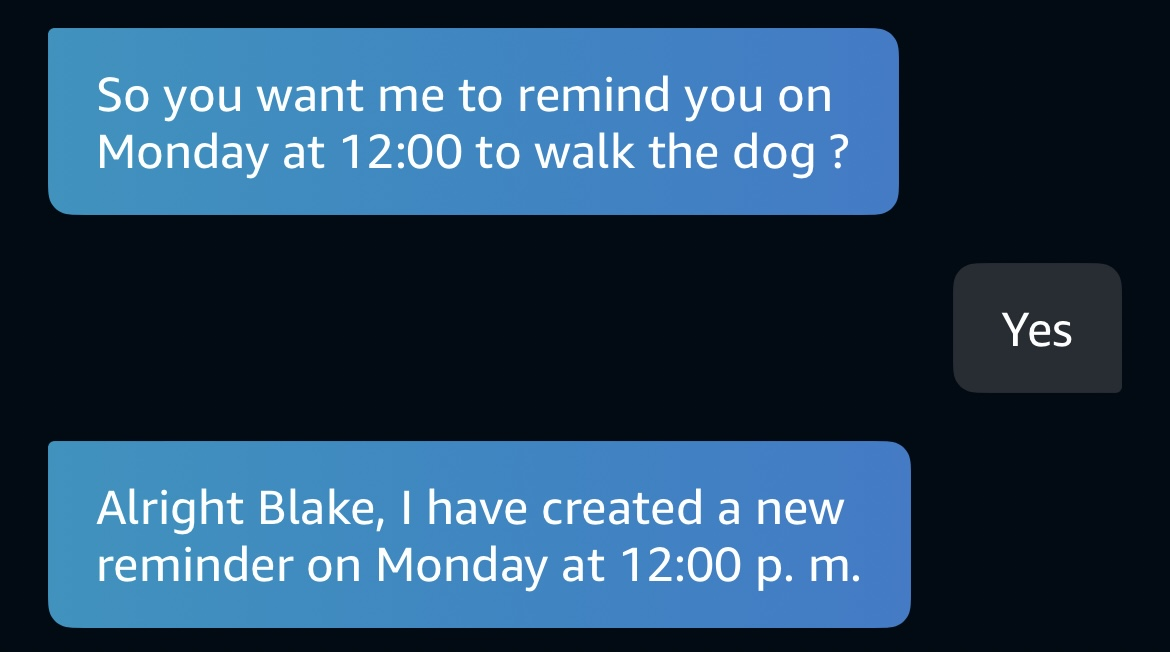
\includegraphics[width=\linewidth * 3/4]{images/createReminder1c.jpg}
\end{center}

Here is another example where the user provides more detail from the very beginning:
\begin{center}
  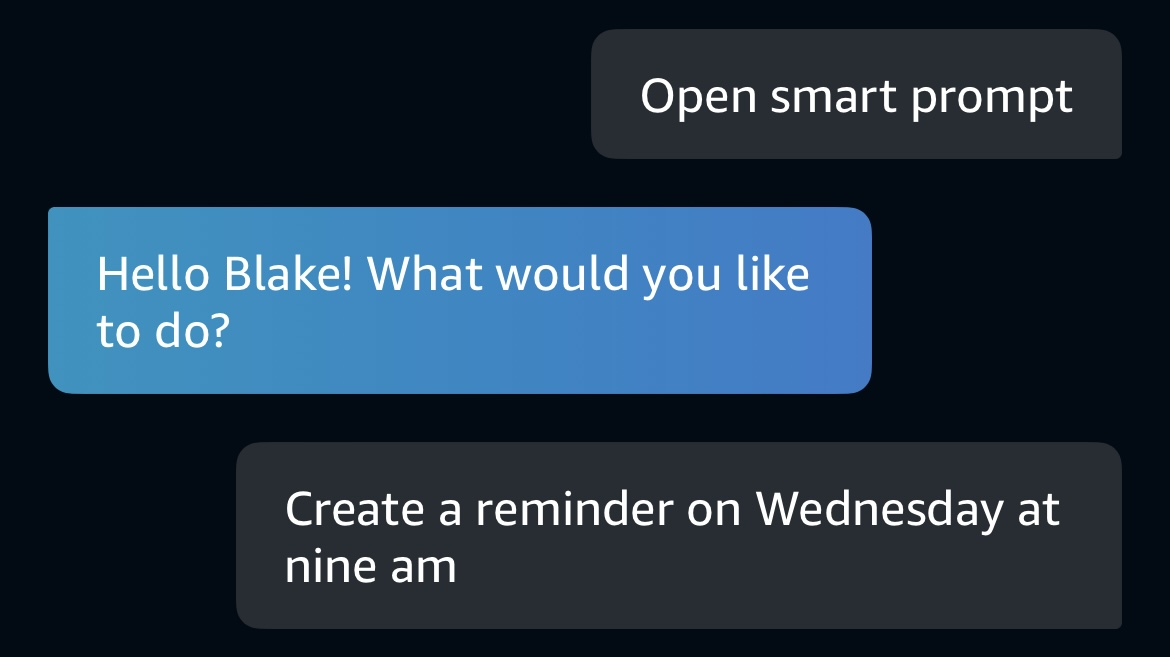
\includegraphics[width=\linewidth * 3/4]{images/createReminder2a.jpg}
\end{center}
\begin{center}
  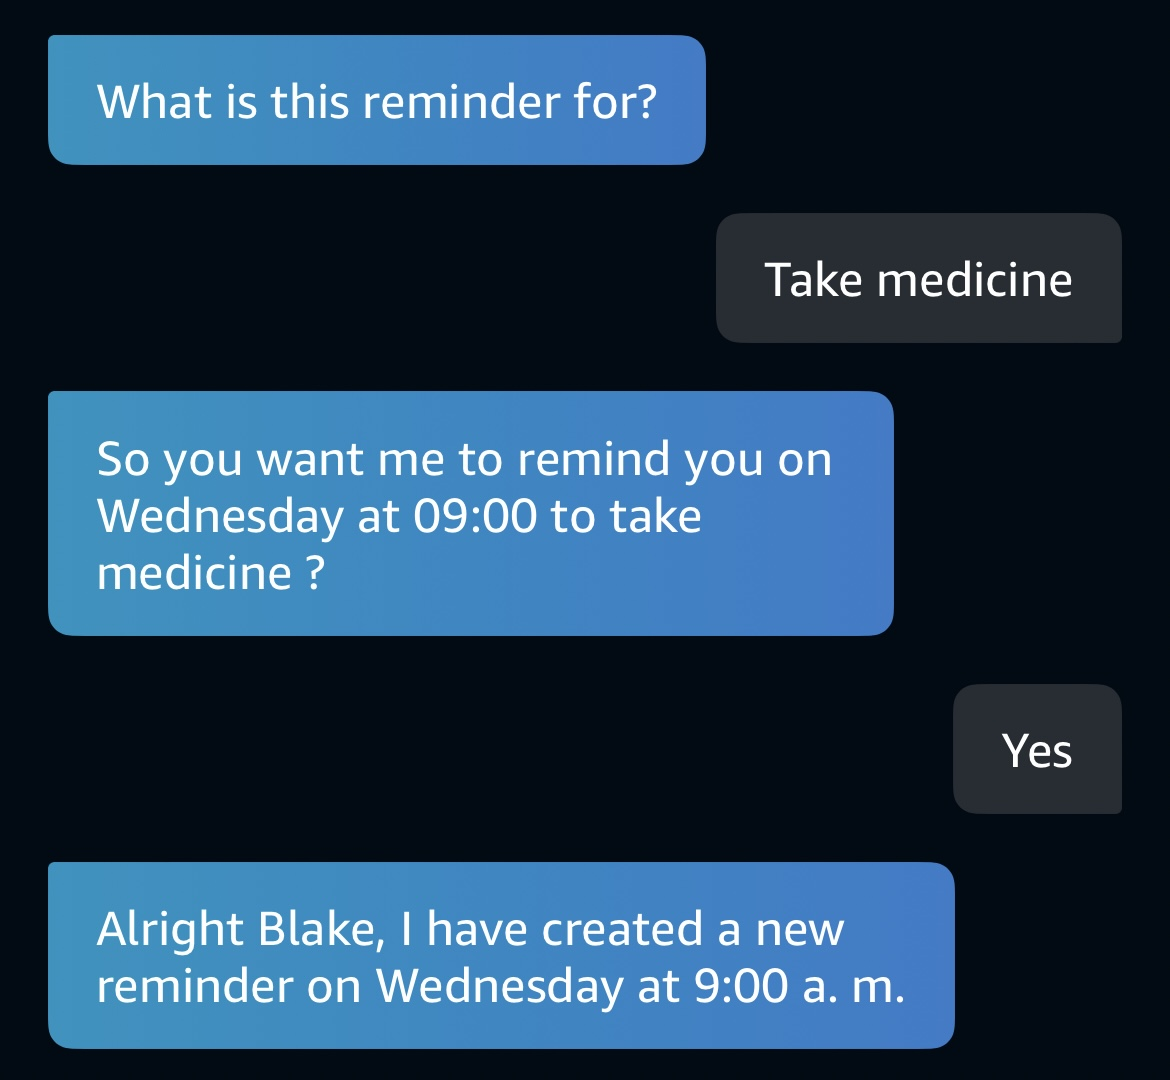
\includegraphics[width=\linewidth * 3/4]{images/createReminder2b.jpg}
\end{center}

Finally, here is an example of the user phrasing the request in a completely different way:
\begin{center}
  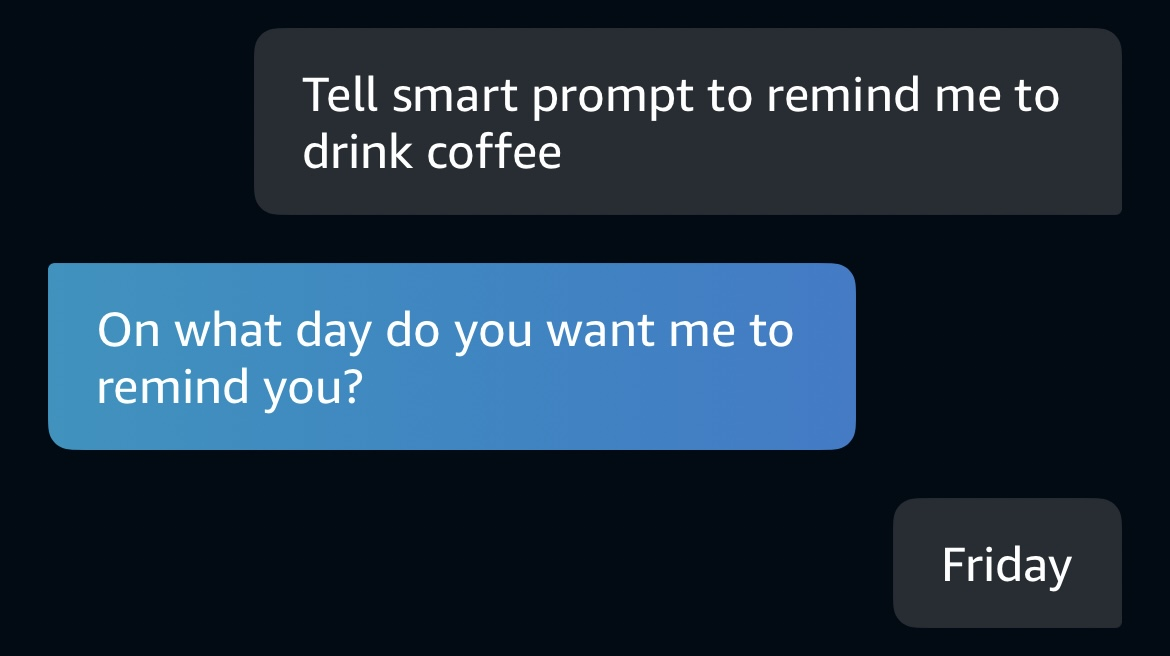
\includegraphics[width=\linewidth * 3/4]{images/createReminder3a.jpg}
\end{center}
\begin{center}
  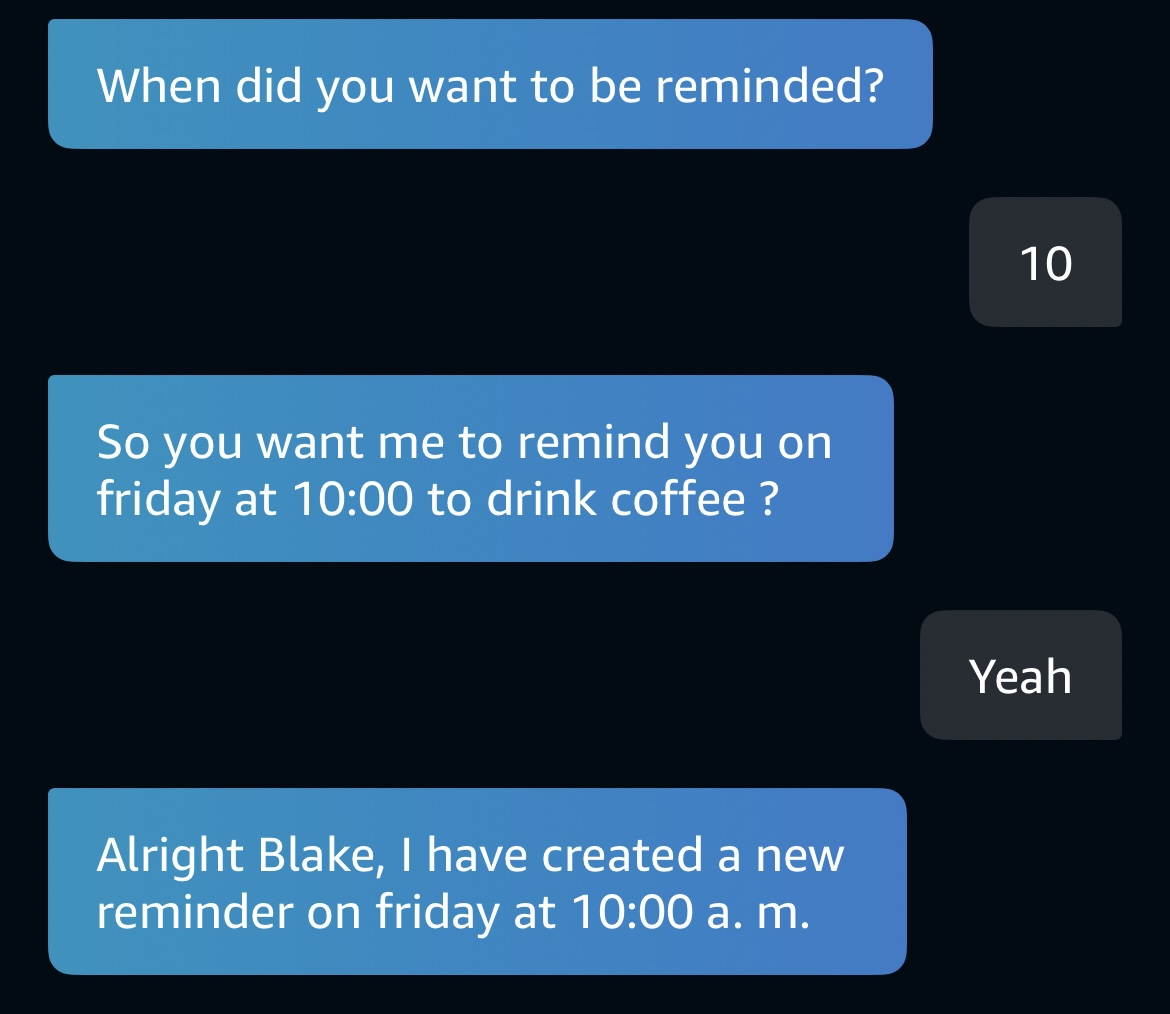
\includegraphics[width=\linewidth * 3/4]{images/createReminder3b.jpg}
\end{center}

\subsubsection{Completed Reminder Intent}

The Completed Reminder Intent is slightly less straight forward, although still what it sounds like: it allows the user to record a reminder as complete. 
There is no required information here, the user simply needs to say something along the lines of "I completed my task". 
Once the user says this and the intent fires, the skill performs some database operations. 
First it checks what reminder is pending (i.e., the last reminder that went off). 
Then it performs some read \& write operations in order to record the task as complete as well as the time of completion. 
Finally, it clears the pending reminder and checks if the reminder completed has an audio file saved. 
If it does, it plays the audio file. 
Otherwise it simply notifies the user that the reminder has been recorded as complete. 

Here is an example of the user completing a reminder:
\begin{center}
  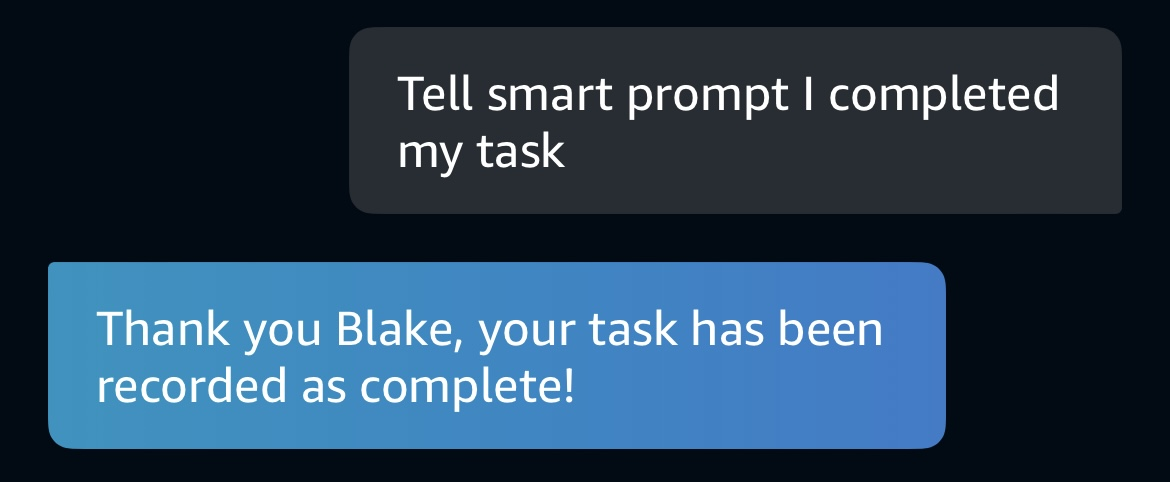
\includegraphics[width=\linewidth * 3/4]{images/completedReminder1.jpg}
\end{center}

For obvious reasons the playing of an audio file cannot be shown here, but if an audio file is stored for a given reminder, it would play in place of this confirmation message. 

Here is an example of the user attempting to complete a reminder when there is nothing to complete:
\begin{center}
  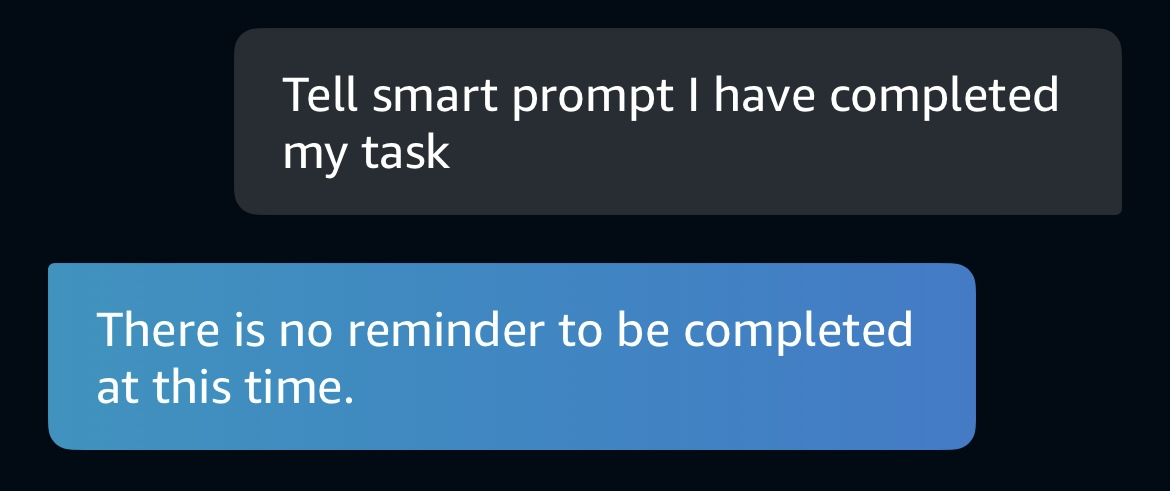
\includegraphics[width=\linewidth * 3/4]{images/completedReminder2.jpg}
\end{center}

\subsubsection{Reminder Started Event}

This event handler, as it sounds, occurs whenever a reminder starts, i.e., right as it goes off. 
Obviously there is no user interaction here (the actual noise of the reminder going off as well as the user asking for it to stop is handled solely by Alexa's built in framework), but there are some database operations that occur here. 
First off, the skill uses the reminder ID to search the database for the reminder data. 
A new "iteration" of the reminder is stored for each week that it occurs, so if it is the first time that reminder is going off that week, a new iteration will be created and the start time of the reminder will be recorded. 
Otherwise, the current iteration will simply be found and the number of snoozes for that iteration will be incremented. 
Finally, this reminder will be entered as the previous reminder in the database, for the purposes required by the Completed Reminder Intent. 

\subsection{Dialog Model}

In case it is easier to follow, here is a diagram showing the flow in which the user interacts with Smart Prompt during the two main intents: 
\begin{center}
  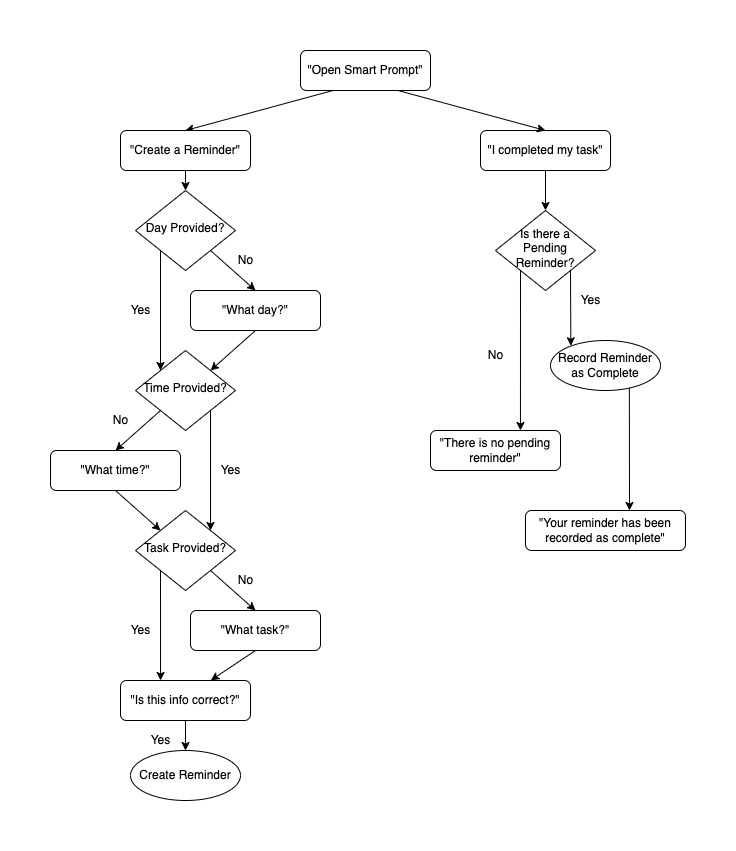
\includegraphics[width=\linewidth * 5/6]{images/dialogModel.jpg}
\end{center}

\subsection{Backend}

The Firebase Realtime Database, being a NoSQL database, is structured more like a large JSON object than anything else. 
At the most global level there is a users list. 
This list is indexed by the user's Alexa ID, such that when the skill needs to access the database it simply uses the user id that it has stored itself. 
Within each user object then exists a reminders list. 
Similarly to the users array, the reminders list is indexed using the Alexa ID of each reminder, again for the same reason as the users ares stored using their Alexa ID. 
Additionally, there exists a previous reminder object stored at the user level in order for the skill to know the pending reminder for each individual user. 
Moving on, each reminder object contains numerous fields. such as the reminder day, time, \& message. 
Each reminder also includes an optional audio file field, which contains the name of an audio file stored in an Amazon S3 bucket (if this field is included, the audio file named will be played when a reminder is recorded as complete).
The last field in each reminder is the iterations list, with each iteration representing the reminder data for any given week. 
Each iteration stores the start time (the exact time the reminder first went off), the completion time (if it was completed), whether not it was completed, and the number of times it went off (i.e., number of snoozes that went off). 

Here is a screenshot of a sample reminder in the database: 
\begin{center}
  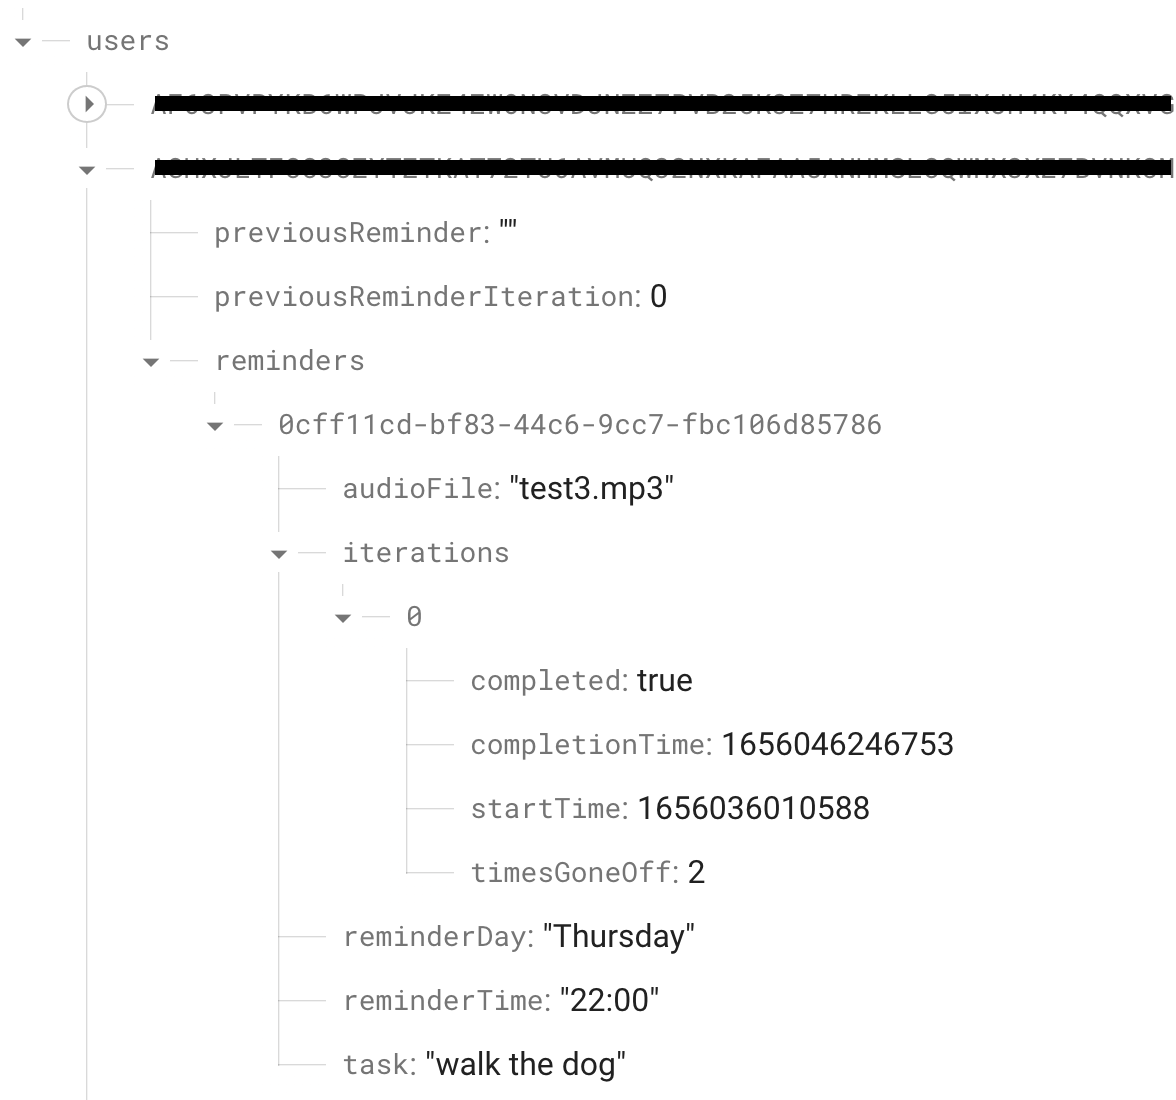
\includegraphics[width=\linewidth * 2/3]{images/databaseEx.png}
\end{center}

\subsection{System Diagram}

Finally, here is a simple system diagram showing each technology used. 
Amazon Alexa is at the core of Smart Prompt and it communicates with Google Firebase in order to store the vast majority of data. 
Amazon S3 is used simply to store the optional audio files to be played at the completion of tasks. 
\begin{center}
  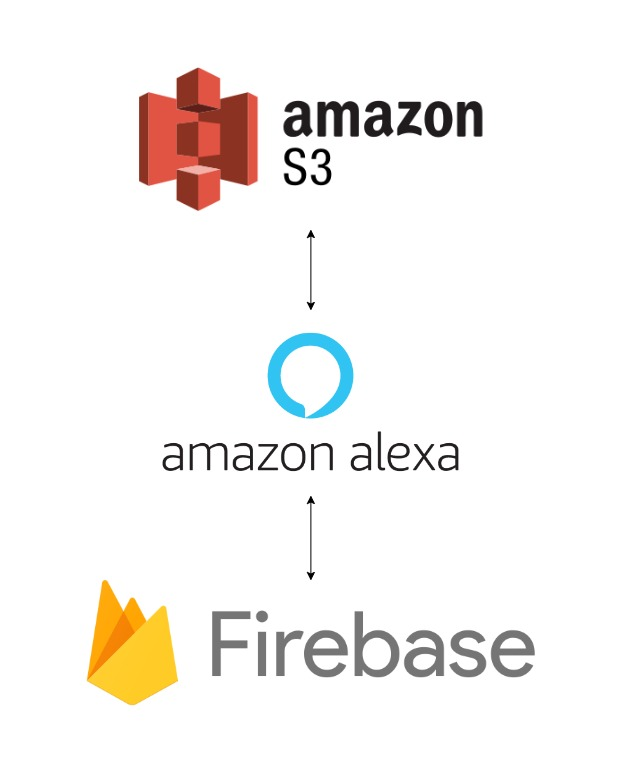
\includegraphics[width=\linewidth * 2/3]{images/systemDiagram.jpg}
\end{center}


\section{Evaluation}

In this section we will examine other projects and commercial solutions related to Smart Prompt, and see how Smart Prompt compares to them. 
Surprisingly, there are no notable \& commercially available solutions that are directly comparable to Smart Prompt, so we will focus on existing Amazon reminders, other general reminder/task management solutions, and other dementia related health solutions (not specifically task management). 

\subsection{Alexa Reminders}

What becomes immediately evident upon researching the topic of Alexa reminders, and even more so specifically for users with memory ailments, is that the reminder system built into every Alexa device remains the king of this category. 
It is, admittedly, a well fleshed out, useful system that would fulfill most peoples wishes when making a reminder. 
However, it does not provide everything we are looking for in our reminder system. 

Let us examine the main features more closely. 
Alexa allows users to create reminders for any sort of time on any sort of interval. 
They can create daily, weekly, monthly, or any sort of recurring reminder. 
They can also create relative reminders, i.e., to be reminded of something an hour from now. 
They can even create location based reminders, such that they are reminded of something upon arriving at a certain location. 
Additionally, once the reminder is created, they can do almost anything with it. 
They can change the time, the message, the day, the details of the recurrence, and pretty much every other detail you can think of (all of this can be edited in the app or via voice controls).
Being reminded of what reminders you may have is straight forward as well. The user can ask, "what reminders do I have today?", or, "when is my next reminder?". 
When the reminder goes off, the user can even ask for it to be snoozed for any amount of time, and if it is a recurring reminder, it will only alter the one instance and not the whole series. 
Essentially, users can create any type of reminder, and viewing, updating, and deleting those reminders is straight forward and thoroughly implemented.  

For the vast majority of users, this is more than what they need or even want. 
However, for our use case, this is lacking in some departments. 
First of all, considering our users will have memory ailments, it would not be easy for them to remember if they completed a reminder or not. 
And when they did, it would still be hard for them to remember exactly when (in case they had snoozed it or took a long time to complete it).
These details are often important for our potential user base. 
For example, one reminder might be related to taking a very important medication, and it would be helpful for the user \& potential caregiver to be able to view whether or not the medication was taken. 
Another example would be if the user is undergoing physical therapy. Considering it might be hard for the user to remember when they performed their necessary exercises, it would be beneficial for the user's doctor to be able to concretely view a record of completion. 
For these reasons, a tracking system of some sort is a basic requirement for our solution, and Alexa is entirely lacking in that department. 
Alexa merely sets of a reminder at a given time and forgets about it from there on out. 
It does not care in the slightest about what happens after the reminder goes off or what the user does in response to the reminder. 

Another, somewhat simpler issue is that Alexa completely lacks personalization. 
For a younger person that is more tech savvy, they are probably happy with a more blunt, to the point Alexa conversation. 
However, our target user base is much older and did not grow up with technology like Alexa. 
Thus, to make using our solution feel less like talking to a robot and more like a personal experience, it is a requirement that it contains personalization. 
Not only would personalization make the transition into using the solution as well as the general experience better, but it would provide more incentive into using the solution and completing your reminders. 
For example, if the solution were able to refer to the user by name and play a custom clip of a family member greeting them upon completing a reminder, then the user would most definitely be more likely to complete a reminder and continue to use our solution than if they simply received nothing but monotone instructions from a device. 

In short, although Alexa has a well built reminder system already, it is lacking some core requirements we are looking for in our solution. 

\subsection{Other Reminder Solutions}

Firstly, let us examine some third party custom Alexa skills related to reminders \& task management. 
Commercially, there is not much. 
When you search for reminders under Alexa Skills or go to the Productivity section, most of what comes up are very niche, specific, simple skills. 
For example, the skill that came up the most was "Stand Up Reminder", a skill built solely to remind you to stand up every 45 minutes. 
Beyond that the most notable skills involve reminding users to drink water, when their friends' birthdays are, and when to do yoga. 
Notably, however, there are a small number of skills attempting to provide a general, non-niche reminder system. 
Although, none of these general reminder skills expand upon the base functionality of Alexa reminders in any way. 
In fact, no skills came up that even matched Alexa's base reminder functionality, they were all even simpler with fewer features. 

Moving away from Alexa for a little, there are countless reminder \& task management systems out there. 

\subsection{Other Memory Ailment Related Solutions}

put anything related to solving a problem for memory ailments here

\subsection{Extras}

put noteworthy things here, i.e., the very similar project that never came to be and the articles about using base Alexa for dementia


\section{Discussion}

Discuss what couldn't be finished, difficulties, next steps, etc. (specifically go into detail about how to implement the auto snoozing)


\section{Conclusion}

Conclusion


\section{Appendix}

\subsection{First Use}

Smart prompt requires permissions in order to create reminders for you and refer to you by your given name. As these are core functionalities of the skill, it will require you to grant them right off the bat.
There are two ways to grant permissions:

\begin{enumerate}
  \item Have Smart Prompt Ask You:
First, launch the skill by simply saying
\begin{center}
"Alexa, open Smart Prompt"
\end{center}
Alexa will then directly ask you to grant permissions. You may approve or decline them, although declining them will simply keep you from using Smart Prompt. Once you approve them, you will have full access to Smart Prompt's features immediately afterwards.
  \item In the Alexa App:
If you prefer to accept the permissions manually you may do so by simply opening the Alexa App (mobile or web), navigating to the Skills menu, then Your Skills, then Smart Prompt, then Settings, and finally you can check off the two required permissions.
As a side note, it is possible to only check off one of the two permissions, although many parts of the skill will be unusable and it will simply request that you grant the necessary permissions.
\end{enumerate}

Simply ensure that both permissions are granted as such:
\begin{center}
  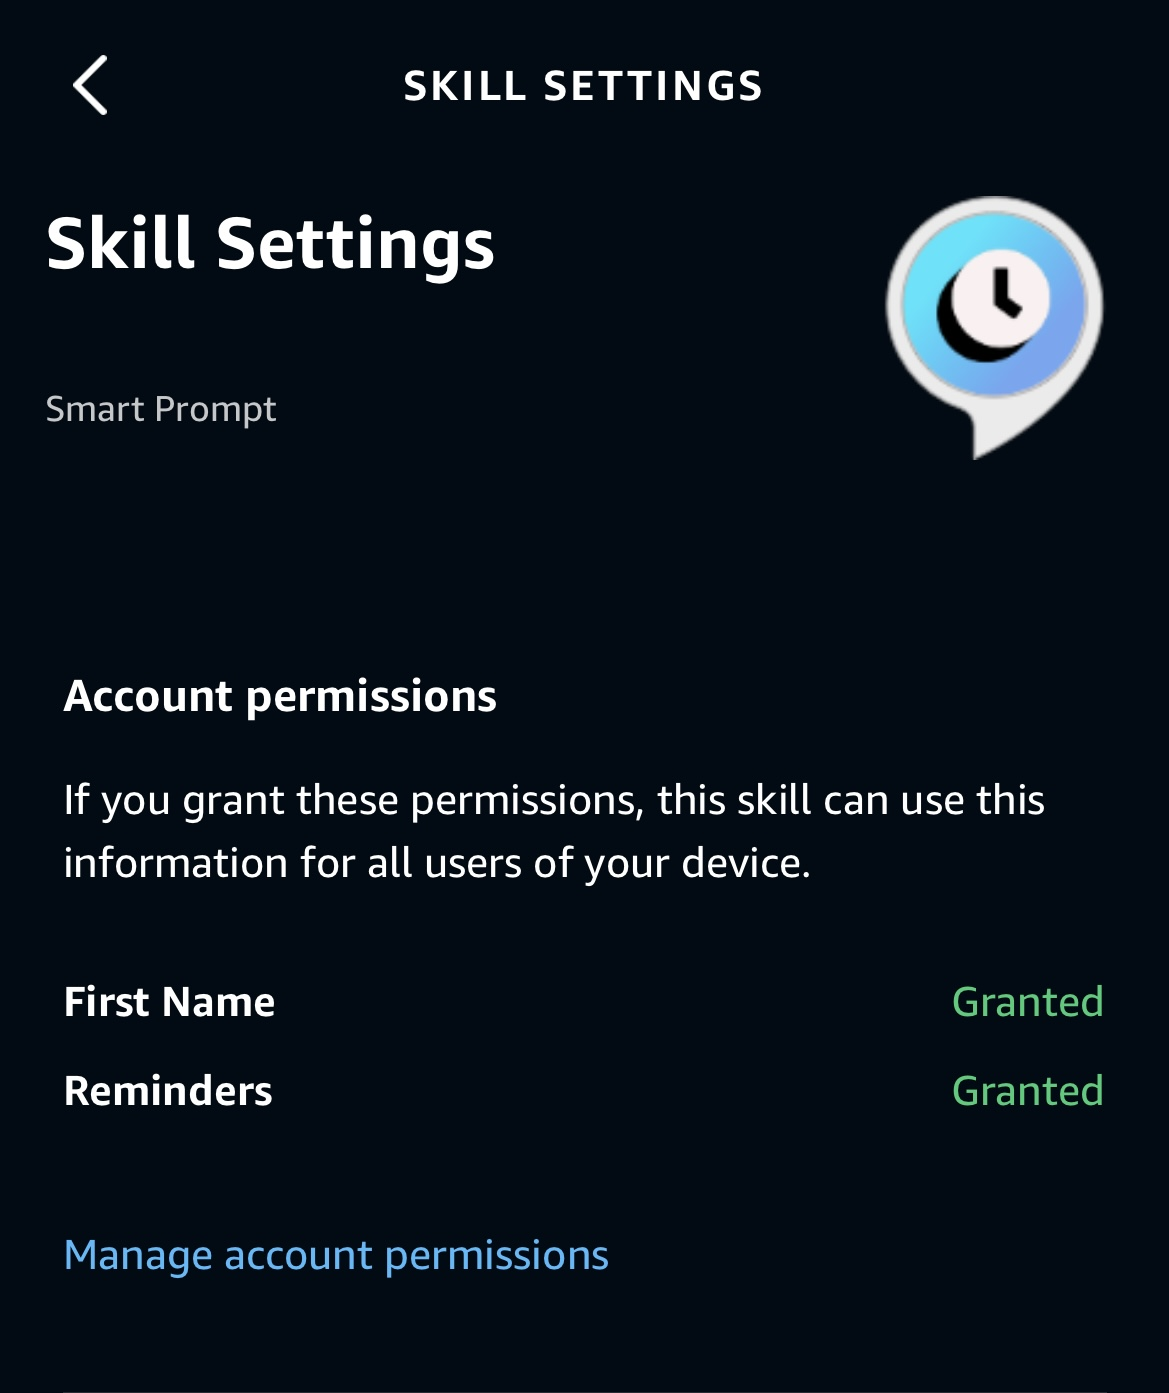
\includegraphics[width=\linewidth * 1/2]{images/skillPermissions.jpg}
\end{center}

\subsection{Creating a Reminder}

To create a new reminder, simply ask Smart Prompt. First, launch Smart Prompt using the same launch phrase listed above, and then say anything along the lines of
\begin{center}
"Create a new reminder"
\end{center}
The skill will then prompt you for three pieces of information one by one:
\begin{itemize}
    \item Day of the Week, i.e., Monday, Tuesday, etc.
    \item Time of Day, i.e., 9:00 a.m., Noon, 10:00 p.m., etc.
    \item Task / Reminder Message, i.e., "Take ", "Walk the dog", "Make Coffee"
\end{itemize}
Once you provide these three pieces of information, Alexa will repeat them to you and ask you to confirm that they are correct. If anything was recorded incorrectly, you may simply say no and restart the process. Otherwise, simply say yes and the reminder will be created.

Additionally, you may also expedite the process by providing the day and time from the start. Just say anything along the lines of
\begin{center}
"Create a new reminder on Monday at noon"
\end{center}
As a side note, it is worth mentioning that you must create the reminder using this method and not throughout the Alexa App. Any reminder created through other means will not be registered with Smart Prompt and will be missing most of the corresponding features.

\subsection{Snoozing a Reminder}

Snoozing a reminder works exactly the same as any other reminder on Alexa. When an alarm goes off, simply say something along the lines of
\begin{center}
"Alexa, snooze that reminder for five minutes"
\end{center}

\subsection{Recording a Reminder as Complete}

As one of the main purposes of Smart Prompt is to be able to track the completion rate of tasks as well as how long they take, it is encouraged to always tell Smart Prompt when you have completed a task it reminded you to do.

To do this, simply launch Smart Prompt and say something along the lines of
\begin{center}
"I have completed my task"
\end{center}
Upon doing so, Smart Prompt will record the previous reminder that went off as complete as well as how long it was since the reminder first went off (The completion record and duration of time is recorded separately per week for each reminder).

As a side note, do not mention the exact task you completed when performing this action. Smart Prompt is simply unable of recognizing the specific task by name at the moment.

\subsection{Deleting/Updating/Managing Reminders}

Deleting, updating, and generally managing reminders can be handled in exactly the same way as any normal Alexa reminder would be handled. The simplest way is through the Alexa App. All of the basic information of a reminder can be viewed and edited from there.
\begin{center}
  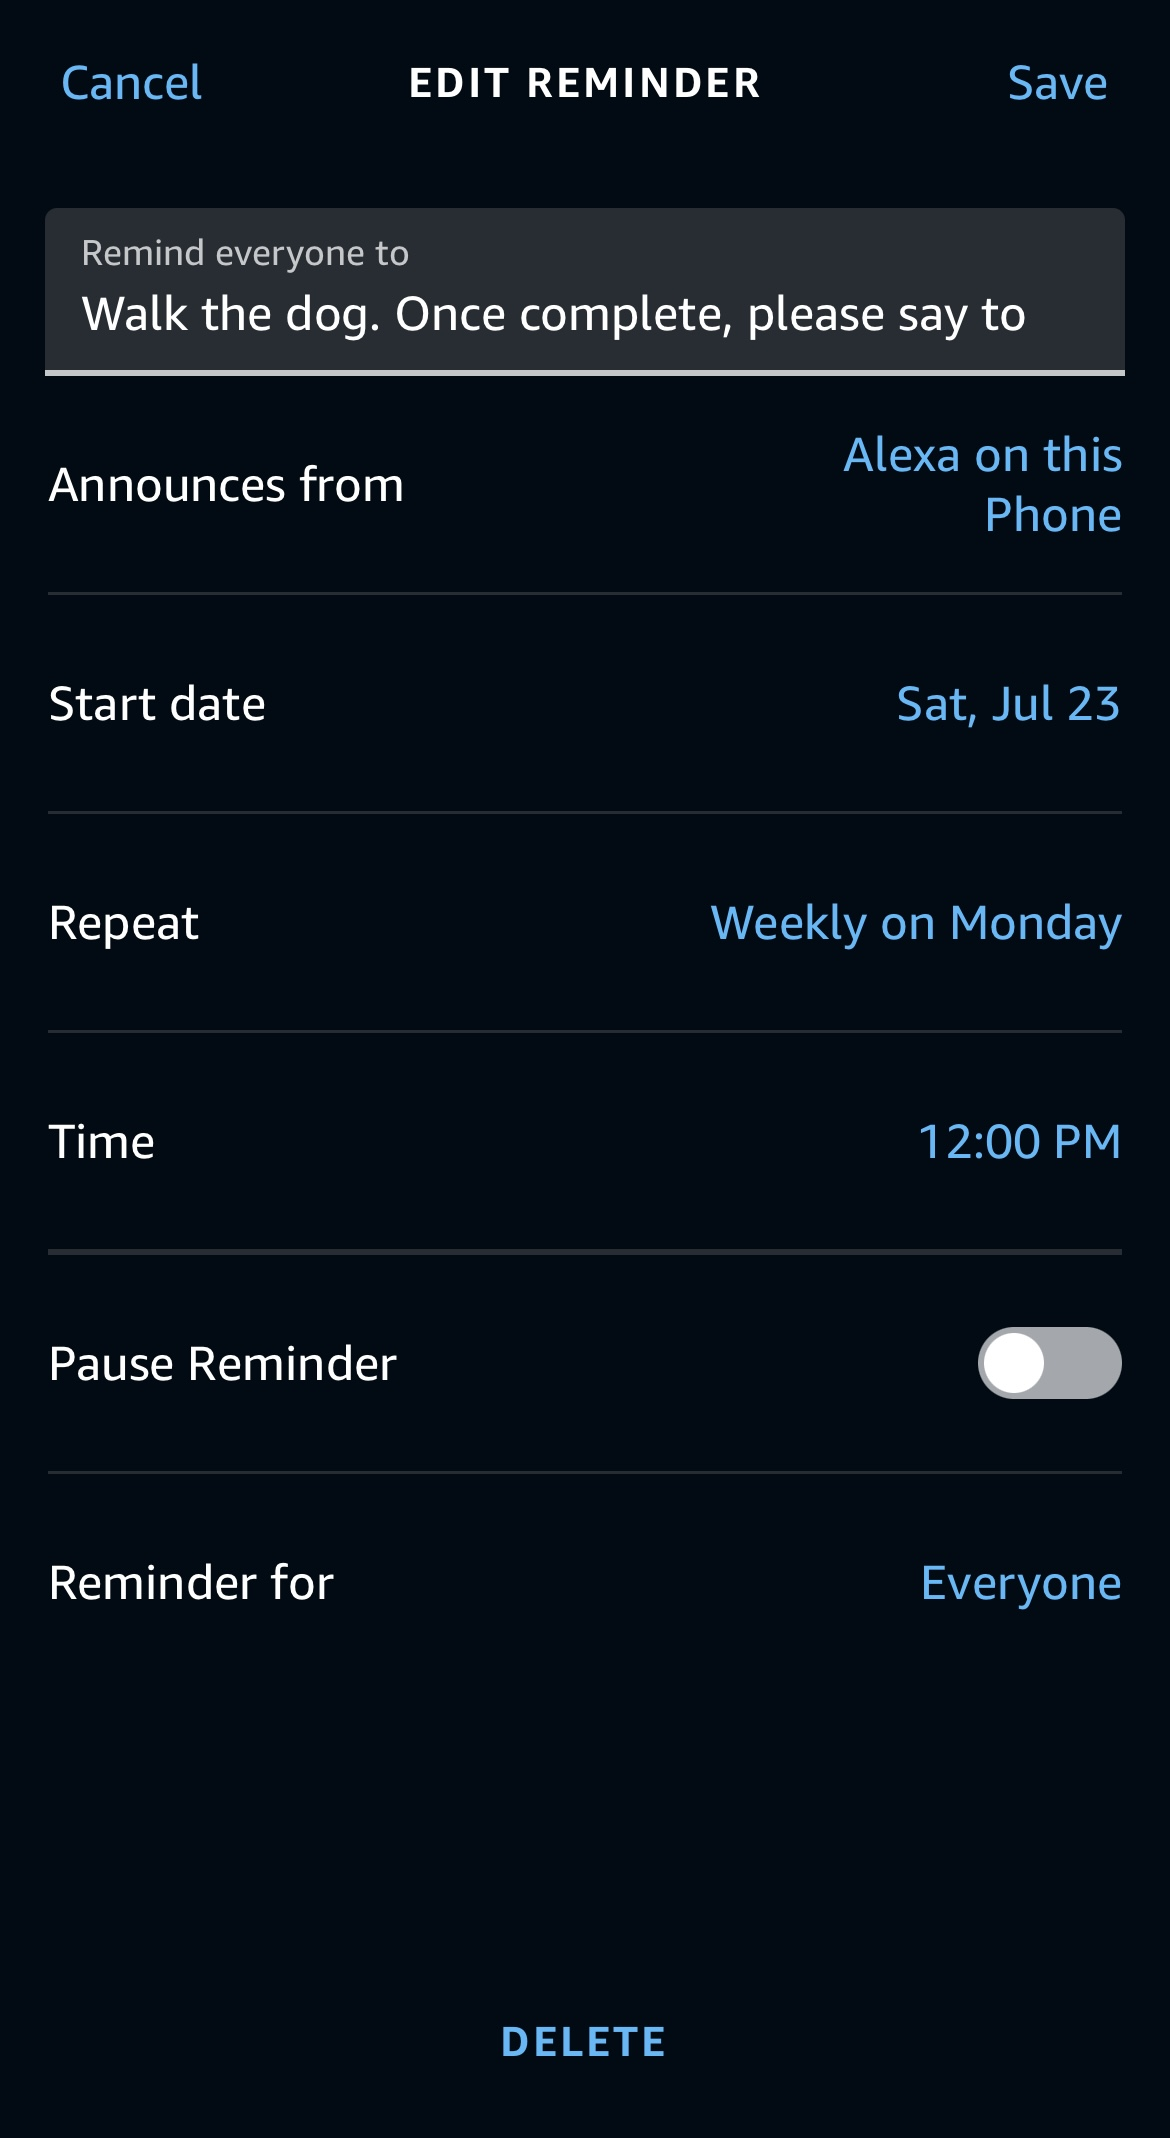
\includegraphics[width=\linewidth * 1/2]{images/inAppReminderSettings.jpg}
\end{center}

Although it is recommended to use the app, you may also ask Alexa about your reminders at any time.
For example, simply say something along the lines of
\begin{center}
"Alexa, what are my reminders"

or 

"Alexa, get rid of my reminder to make coffee"
\end{center}
Be mindful when doing this, however, as Alexa itself will not directly differentiate between Smart Prompt reminders and its own reminders.

\subsection{Formatting \& Uploading an Audio File for Playback}

As mentioned prior, one optional component of Smart Prompt is to have a custom audio file play when you record a task as complete. Anything from a favorite song to a clip of a loved one offering congratulatory words, whatever motivates the user to complete their task can be played. There are two steps to setting this up.

\begin{enumerate}
  \item Audio File Formatting: 
  Any standard MP3 file can be used with Smart Prompt, but there is some formatting it must go through prior to uploading it, otherwise Alexa will simply not play it. Amazon themselves provide two methods, a command line tool as well as Audacity (a popular \& free audio editing software), but it is highly recommended to use Audacity as it is more straight-forward and reliable. Essentially, you just need to open your MP3 file in Audacity, set the project rate to 16,000, go to File, then Export, set the save type to MP3, set the bit rate mode to constant, and finally set the quality to 48 kbps. With all of that done you can save this new MP3 file and the formatting is complete.
\begin{center}
  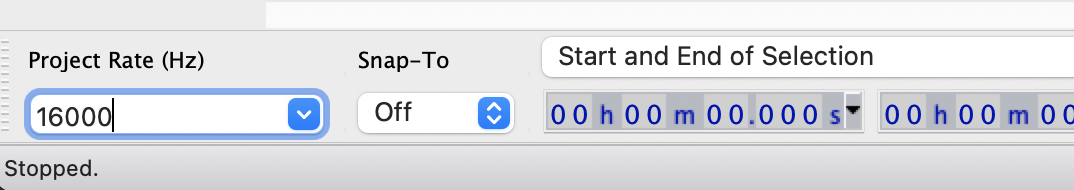
\includegraphics[width=\linewidth * 3/4]{images/audacityProjectRate.png}
\end{center}
\begin{center}
  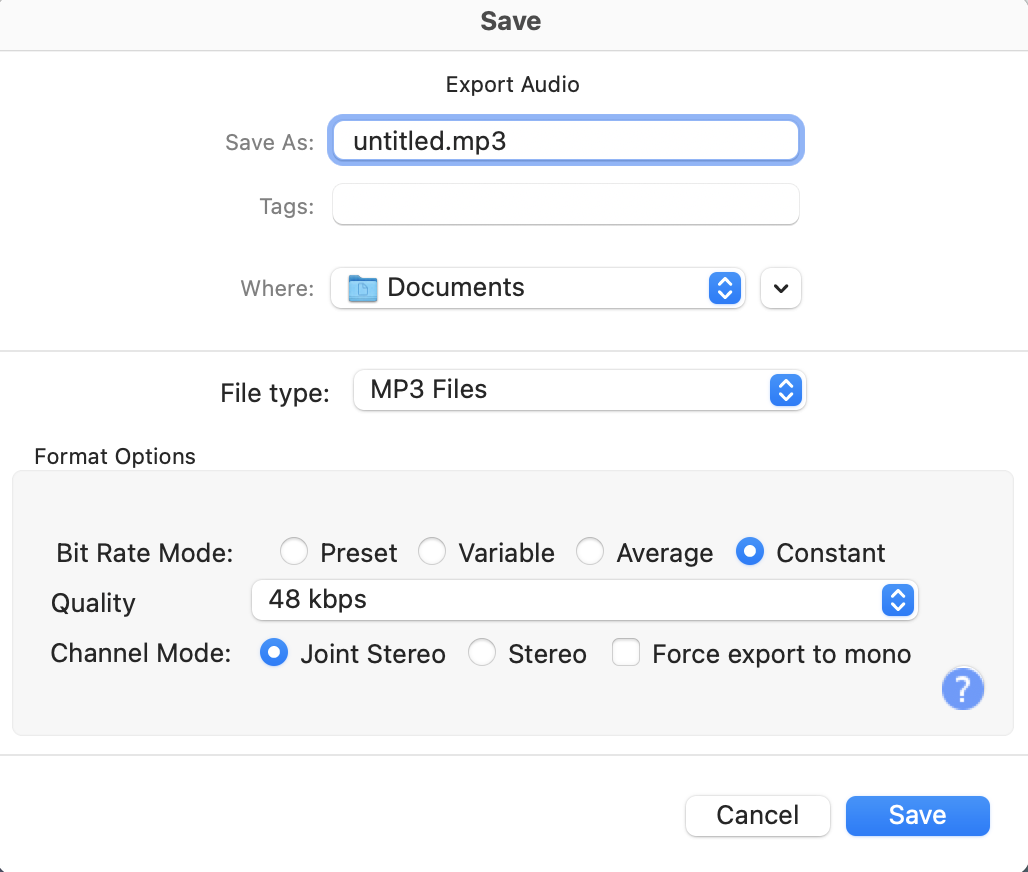
\includegraphics[width=\linewidth * 1/2]{images/audacityExportSettings.png}
\end{center}
  
  \item Uploading to S3 \& Linking to DB:
  With your formatted MP3 in hand, there are only two things left to do. First, you must upload the file to the Amazon S3 Bucket tied to Smart Prompt. To do this, simply open Smart Prompt in the Amazon Developer Console, navigate to the code tab, and click on S3 Storage in the toolbar at the top. This will open the S3 Management Console in a new tab, and from here you may simply click upload and drag and drop your MP3 file.
\begin{center}
  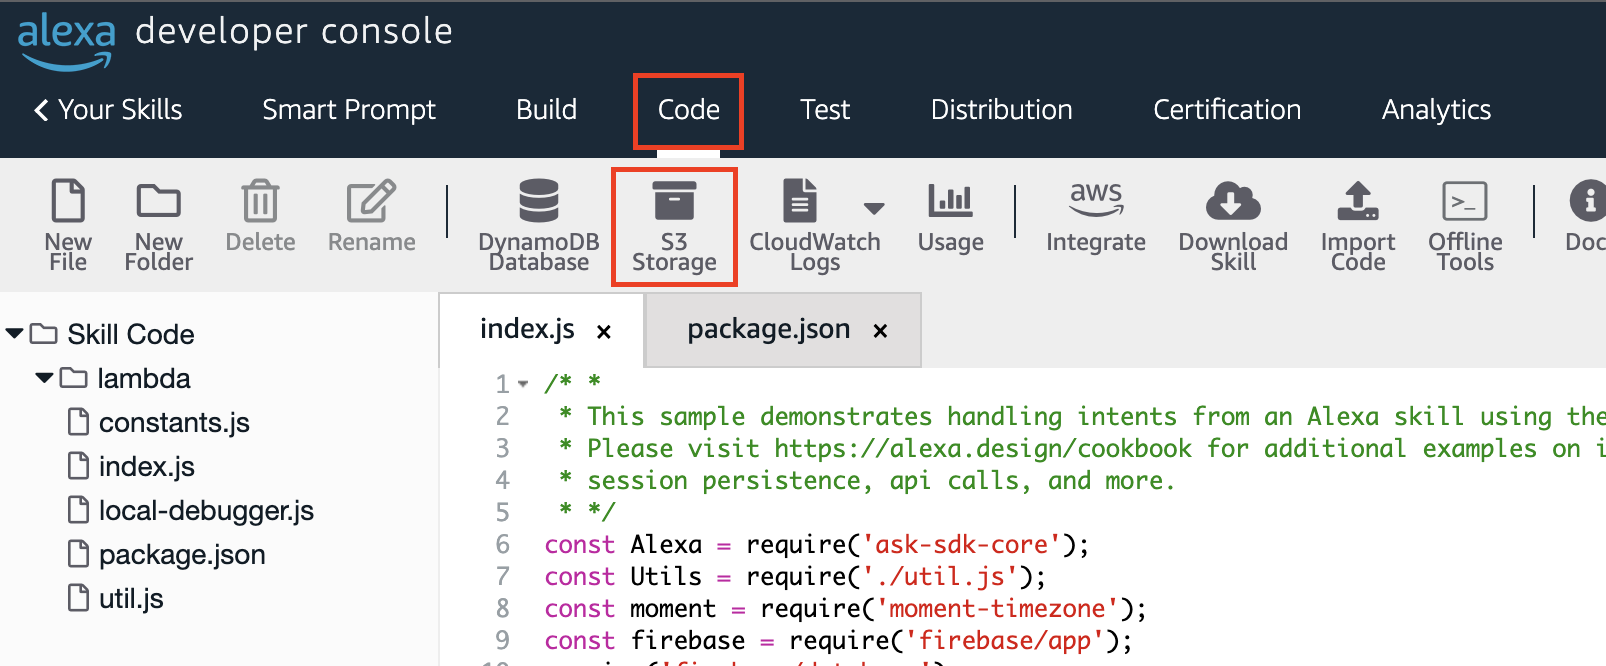
\includegraphics[width=\linewidth * 3/4]{images/s3Location.png}
\end{center}

Finally, you just need to add the MP3 file name to whichever reminders you would like it to play for in the database. To do this, open Smart Prompt in the Firebase Console and navigate to the Realtime Database. From here, find your user and expand it, and then find your reminder and expand it. Then, simply add the following field to the reminder object
\begin{center}
audioFile: $<file name>.mp3$
\end{center}
Make sure the field name is spelled correctly as well as the file name, and then you are good to go. The next time you record this reminder as complete, the audio file will be played as a reward. You may also add this audio file to as many reminders as you would like.
\begin{center}
  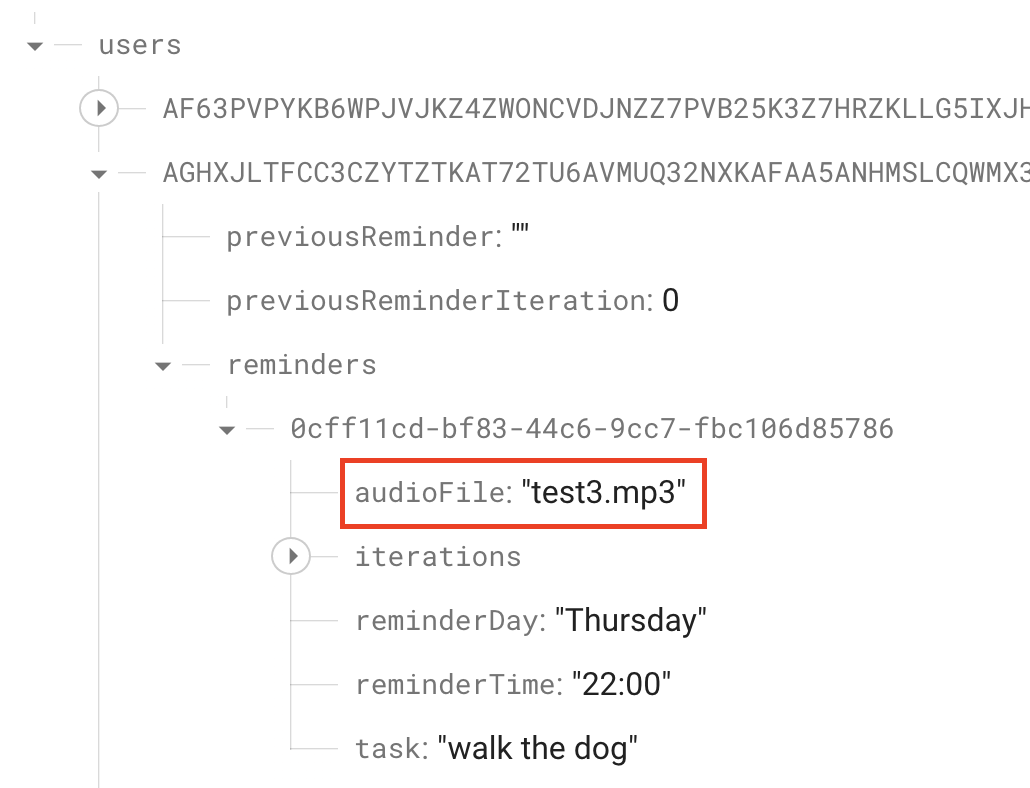
\includegraphics[width=\linewidth * 1/2]{images/audioFileDBField.png}
\end{center}
\end{enumerate}
As a final side note, an easier, more streamlined, and more secure way of uploading and managing audio files will be implemented in the future.

\subsection{Extras}

One thing worth noting is that, as with any skill, the launch sequence can be expedited by simply saying,
\begin{center}
"Alexa, tell $<skill name>$ $<intent>$"
\end{center}
For example, to quickly tell Smart Prompt you have completed a task, simply say,
\begin{center}
"Alexa, tell Smart Prompt I have completed the task"
\end{center}
This can make navigating Smart Prompt, or any other skill, much quicker and simpler. The only thing to take note of with this is that if you do this before granting permissions, the intent will simply not work and it will request that you grant permissions.

\begin{thebibliography}{00}
\bibitem{b1} Alisha Pradhan, Amanda Lazar, and Leah Findlater. 2020. Use of Intelligent Voice Assistants by Older Adults with Low Technology Use. ACM Trans. Comput.-Hum. Interact. 27, 4, Article 31 (August 2020), 27 pages. https://doi.org/10.1145/3373759
\bibitem{b2} Beaney, P., Kalirai, H.S. and Chambers, R. (2020), “Alexa… what pills do I need to take today?”. Prescriber, 31: 20-23. https://doi.org/10.1002/psb.1849
\bibitem{b3} Jesús-Azabal, M., Medina-Rodríguez, J.A., Durán-García, J., García-Pérez, D. (2020). Remembranza Pills: Using Alexa to Remind the Daily Medicine Doses to Elderly. In: García-Alonso, J., Fonseca, C. (eds) Gerontechnology. IWoG 2019. Communications in Computer and Information Science, vol 1185. Springer, Cham. https://doi.org/10.1007/978-3-030-41494-8\_15
\bibitem{b4} Plassman B, L, Langa K, M, Fisher G, G, Heeringa S, G, Weir D, R, Ofstedal M, B, Burke J, R, Hurd M, D, Potter G, G, Rodgers W, L, Steffens D, C, Willis R, J, Wallace R, B: Prevalence of Dementia in the United States: The Aging, Demographics, and Memory Study. Neuroepidemiology 2007;29:125-132. doi: 10.1159/000109998
\bibitem{b5} Ruggiano N, Brown E, Roberts L, Framil Suarez C, Luo Y, Hao Z, Hristidis V
Chatbots to Support People With Dementia and Their Caregivers: Systematic Review of Functions and Quality
J Med Internet Res 2021;23(6):e25006
URL: https://www.jmir.org/2021/6/e25006
DOI: 10.2196/25006
\bibitem{b6} Shu, S., \& Woo, B. K. (2021). Use of technology and social media in dementia care: Current and future directions. World journal of psychiatry, 11(4), 109–123. https://doi.org/10.5498/wjp.v11.i4.109
\bibitem{b7} Wolters, M. K., Kelly, F., \& Kilgour, J. (2016). Designing a spoken dialogue interface to an intelligent cognitive assistant for people with dementia. Health Informatics Journal, 854–866. https://doi.org/10.1177/1460458215593329
\end{thebibliography}

\end{document}